\documentclass[20pt,margin=1in,innermargin=-4.5in,blockverticalspace=-0.25in]{tikzposter}
\geometry{paperwidth=42in,paperheight=30in}
\usepackage[utf8]{inputenc}
\usepackage{amsmath}
\usepackage{amsfonts}
\usepackage{amsthm}
\usepackage{amssymb}
\usepackage{mathrsfs}
\usepackage{graphicx}
\usepackage{adjustbox}
\usepackage{enumitem}
\usepackage[backend=biber,style=numeric]{biblatex}
\usepackage{emory-theme}
\usepackage[final]{pdfpages}

\usepackage{mwe} % for placeholder images

\addbibresource{refs.bib}

% set theme parameters
\tikzposterlatexaffectionproofoff
\usetheme{EmoryTheme}
\usecolorstyle{EmoryStyle}

\title{EZ-AR: An Immersive AR Tool For Advertisements}
\author{Jian Liao, Igor Pieters, Monty Bechir, Nathan Chua and Rakheem Dewji}
\institute{Department of Computer Science, University of Calgary\\
            CPSC~481~Human-Computer~Interaction}
\titlegraphic{
\includegraphics[width=0.20\textwidth]{logo.png}}

\begin{document}
\maketitle
\centering
\begin{columns}
    \column{0.32}
    \block{Our Objectives}{
         EZ-AR is an open-end and innovative way to advertise by using AR to interact with end users in order to promote businesses eventually. The normal advertisements lack interactions with people and will take up unnecessary resources such as physical sites and human resources. Our motivation is to cut off the unnecessary sections of the current way of advertisements and offer a more interactive way to connect potential customers with the products directly and finally to promote the business, which is considered to be B2C business model.
    }
    
    \block{Solution Stack}{
         We present our solution stack in the following figure. Our main goals of this project is providing an SaaS (Software as a Service) service to the business owner as well as end users. In this project, we try to use advanced techniques to build the cross-platform mobile application using Flutter\cite{cite:1}~released by Google in 2018. We also use a full-stack framework in our web application including React as front-end, Node.js as back-end and PostgreSQL as our database. The whole web application is deployed to Heroku.
         
         \begin{tikzfigure}[Solution Stack]
            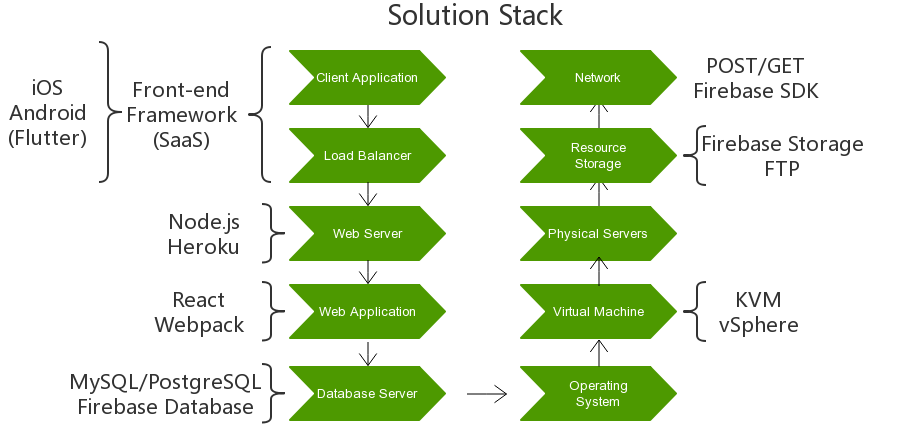
\includegraphics[width=1.0\linewidth]{solution_stack.png}
        \end{tikzfigure}
    }
    
    \block{Database Class Diagram}{
         \begin{tikzfigure}[Database Class Diagram]
            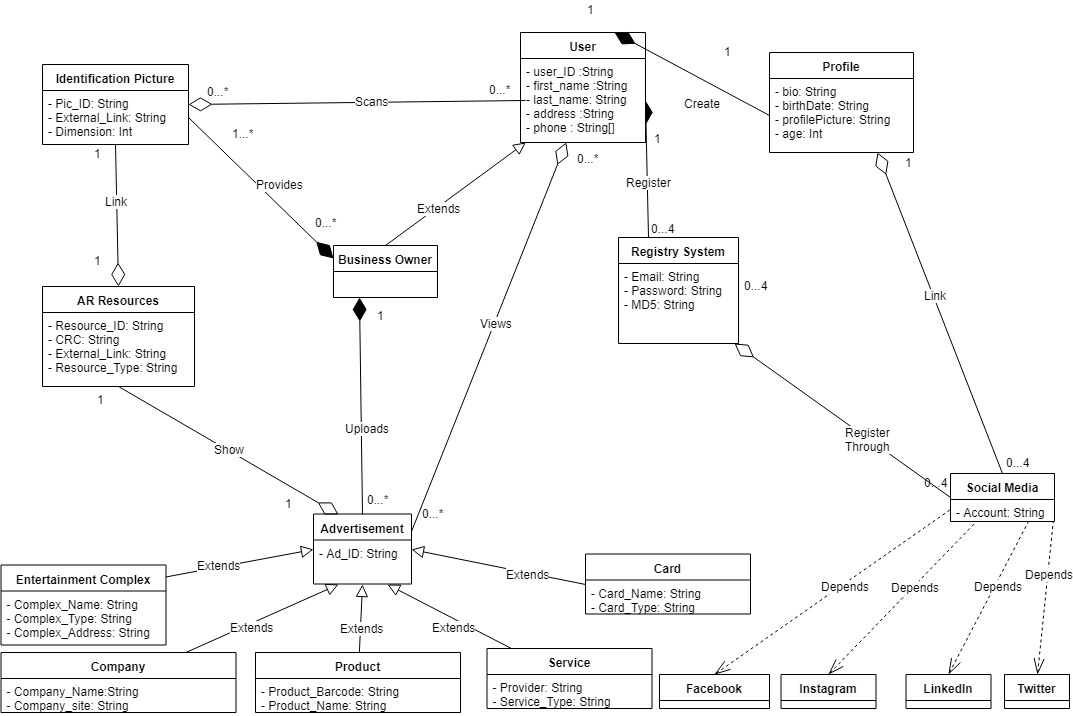
\includegraphics[width=0.78\linewidth]{Class.png}
        \end{tikzfigure}
    }


    \column{0.36}
    \block{EasyAR Engine}{
        The Augmented Reality part is implemented with the SDK from EasyAR\texttrademark \cite{cite:2}. We would require the identification pictures from the business owners and upload them to our cloud server as well as the associated AR resources such as videos, pictures and 3D models.
        
        \begin{tikzfigure}[Block Diagram of EasyAR]
            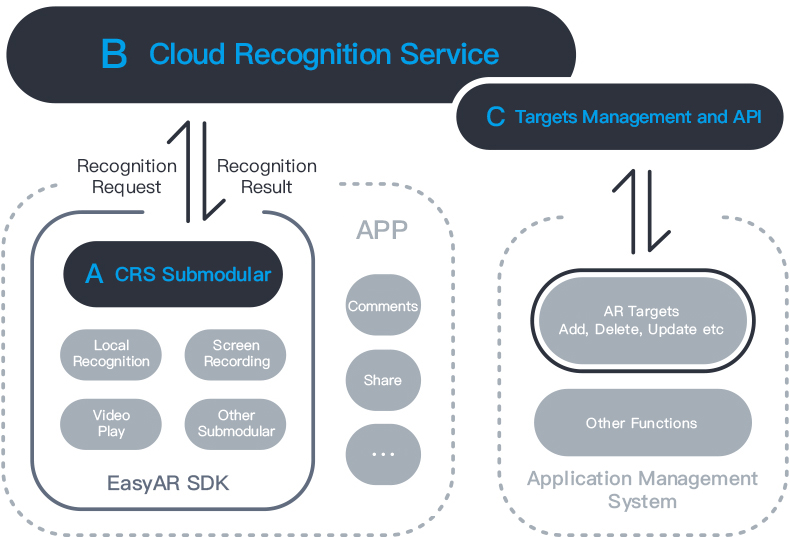
\includegraphics[width=0.9\linewidth]{EasyAR.jpg}
        \end{tikzfigure}
    }
    
        \block{Flutter: Cross-Platform Solution}{
        We use Flutter to develop a cross-platform mobile applications. However, we encounter a technical problem which is AR requires directly hardware interaction. So we design a solution to communicate with native code through MethodChannel\cite{cite:3}.
        
        \begin{tikzfigure}[Flutter Framework]
            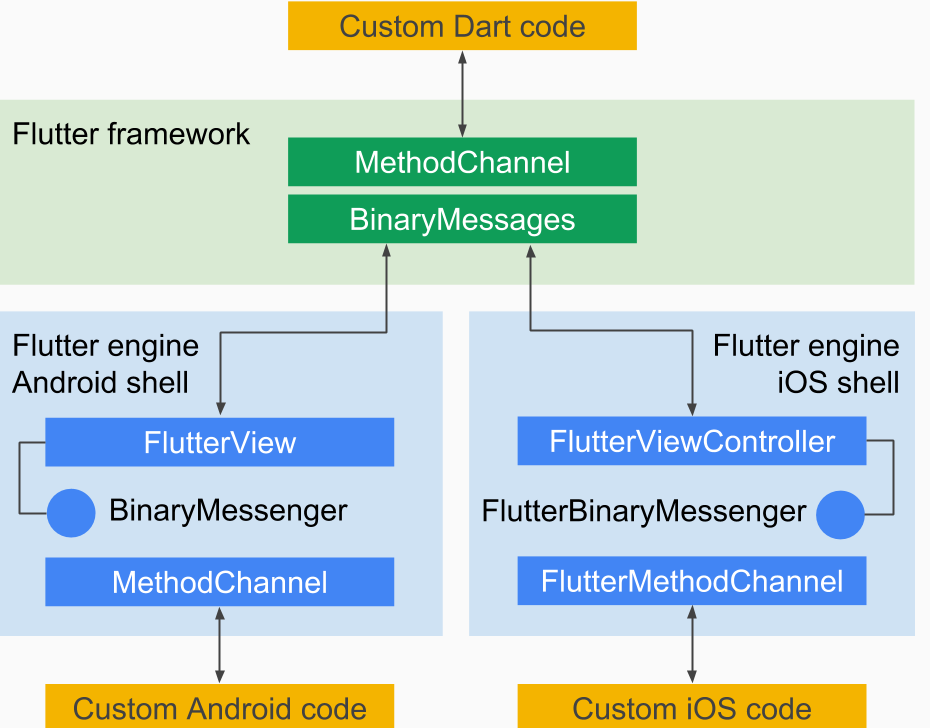
\includegraphics[width=0.7\linewidth]{flutter.png}
        \end{tikzfigure}
        
     
    }

    \column{0.32}

    
    \block{Sequence Diagrams}{
       \begin{tikzfigure}[Users Scan Products]
            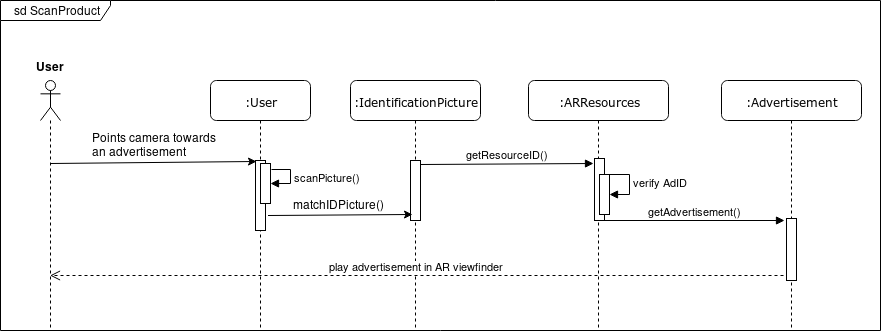
\includegraphics[width=0.65\linewidth]{Sequence2.png}
        \end{tikzfigure}
        
        \begin{tikzfigure}[Users Creat Advertisements]
            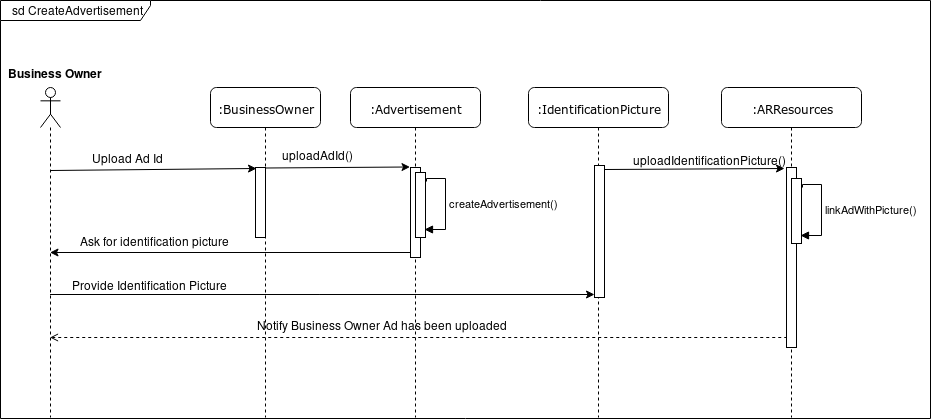
\includegraphics[width=0.65\linewidth]{sequenee3.png}
        \end{tikzfigure}
    }
    
    \block{Design Methods}{
       We decided to conduct two user research methods: Fly on the wall (Look) -> Interview (Ask). We chose Fly on the Wall because it allows us to monitor and make key observations on how a user may interact with a very raw, beta version of our application.
        
        \begin{tikzfigure}[Design Methods]
            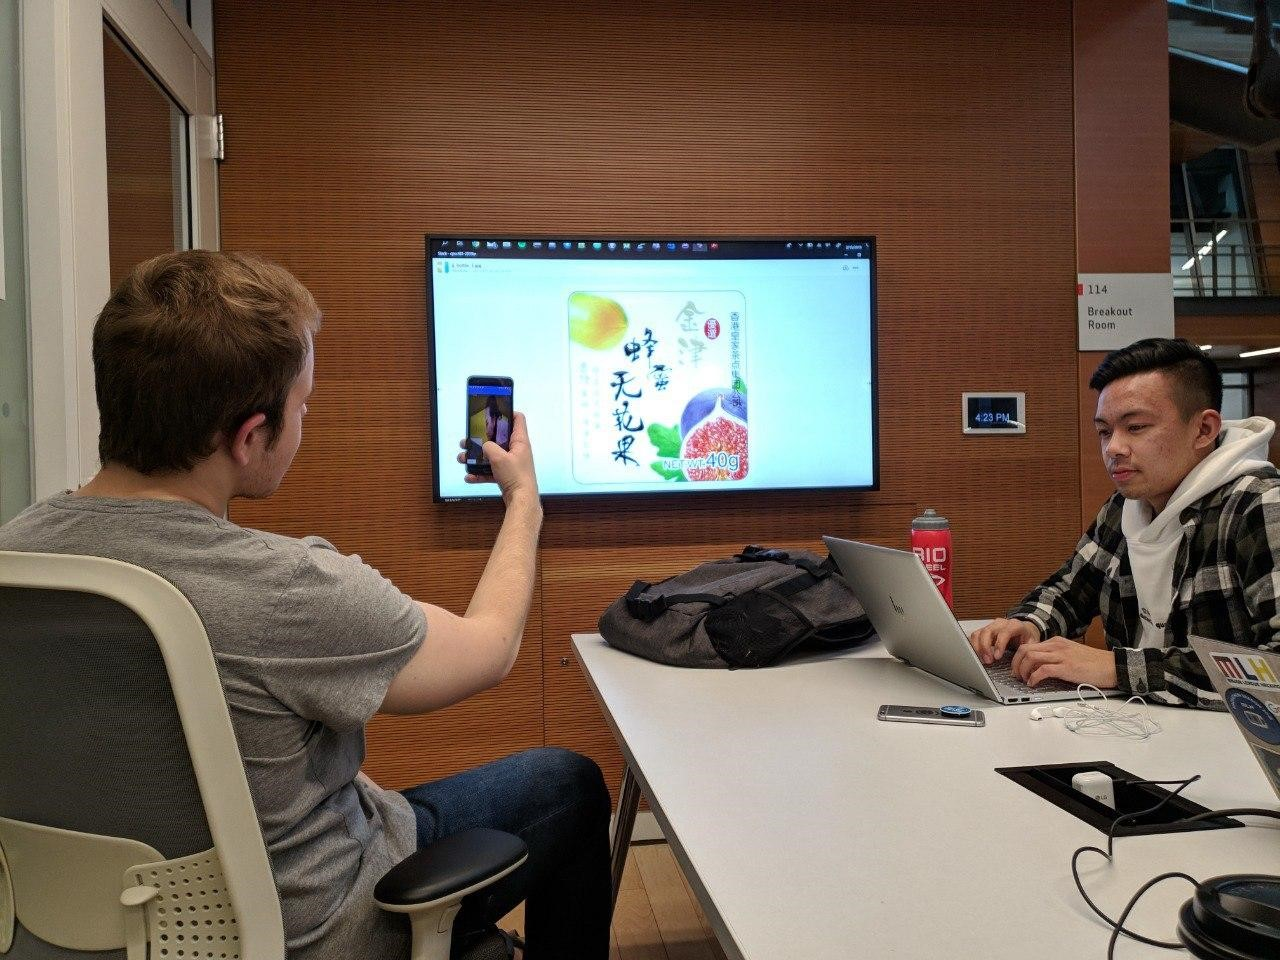
\includegraphics[width=0.55\linewidth]{methods.jpg}
        \end{tikzfigure}
    }

    
    \block{References}{
        \vspace{-1em}
        \begin{footnotesize}
        \printbibliography[heading=none]
        \end{footnotesize}
    }
\end{columns}
\end{document}